\setcounter{page}{1}
\artigofalse
\chapter{General introduction}
\label{chap:introduction}
%\usepackage[utf8]{inputenc}


\section{Background and motivation}

\subsection{Demand for soil information}
\label{sec:intro-demand}

Soil modellers/mappers have complained for many years about the lack of government funding, not only
in Brazil \cite{Dalmolin1999,Ker1999,KerEtAl2003,Mendonca-SantosEtAl2003,Ramos2003,Espindola2008}, but in
many countries around the world \cite{Basher1997,HarteminkEtAl2008,Grunwald2009,SanchezEtAl2009,Finke2012}.
They pointed out several reasons to explain the general lack of interest in soil information by governments
after the 1980's. But all of them seem to agree on one point: cutting down the budget for soil
modelling/mapping fundamentally was an economic decision in which the general public was not given the
chance to participate \cite{SamuelRosa2012}.

The soil science landscape has changed dramatically since the last decade. Soil science is now 
experiencing a period of renaissance \cite{HarteminkEtAl2008}. Soils are back on the agenda 
\cite{Kempen2011}. Soil is now a hot topic. For example, the United Nations 
(\href{http://www.un.org/apps/news/story.asp?NewsID=49520#.VnremV6alz0}{UN}) declared 5 December 
the World Soil Day and 2015 the International Year of Soils \cited{in an effort to raise awareness 
and promote more sustainable use of this critical resource}. A global consortium, the 
\href{http://www.globalsoilmap.net/}{GlobalSoilMap}, was created with the goal of producing 
\cited{a new digital soil map of the world using state-of-the-art and emerging technologies}. 
The Food and Agriculture Organization (\href{http://www.fao.org/index_en.htm}{FAO}) launched a 
Global Soil Partnership (\href{http://www.fao.org/globalsoilpartnership/}{GSP}) for 
\cited{leading to the adoption of sustainable development goals for soils}. The International 
Union of Soil Sciences (\href{http://www.iuss.org/index.php?article_id=525}{IUSS}) created a working group,
funded by the United States Department of Agriculture 
(\href{http://www.nrcs.usda.gov/wps/portal/nrcs/main/soils/survey/class/}{USDA}) to develop a 
Universal Soil Classification System, \cited{a common language to describe soils that can be used 
internationally}. An Intergovernmental Technical Panel on Soils 
(\href{http://www.fao.org/globalsoilpartnership/intergovernmental-technical-panel-on-soils/}{ITPS})
was composed, counting with soil experts from all regions of the world \cited{to provide 
scientific and technical advice and guidance on global soil issues to the Global Soil Partnership}.
The \href{http://www.gatesfoundation.org/what-we-do/global-development/agricultural-development}{Bill 
\& Melinda Gates} foundation handed out an \SI{18}[\$]~million grant \cited{to map most parts in 
Sub-Sahara Africa, and make all Sub-Saharan Africa data available}. The International Soil 
Reference and Information Centre (ISRIC) launched its Global Soil Information Facilities 
(\href{http://www.isric.org/projects/global-soil-information-facilities-gsif}{GSIF}), a 
\cited{framework for production of open soil data}. In Brazil, soil scientists created the 
Brazilian Network for Research in Digital Soil Mapping (\href{https://goo.gl/m8QWUm}{RedeMDS}) with 
the objective of \cited{generating synergy among Brazilian soil scientists to advance the 
research in digital soil mapping}. And the Federal Court of Accounts held a 
\href{https://www.governancadosolo.gov.br/}{Soil Governance Conference}, where a new National 
Program for Soil Survey and Interpretation of Brazil (\href{https://goo.gl/zbMK24}{PRONASOLOS}) was 
announced.

Most soil modellers/mappers seem to agree that there is a \q{renewed recognition} of the importance 
of soils for humanity and the environment, a global understanding that soil information is needed to solve 
those that have been named as the five major problems of our time: food insecurity, climate change, 
environmental degradation, water scarcity, and threats to the biodiversity \cite{SanchezEtAl2009}. 
This \q{renewed recognition} would be the reason for an increasing worldwide societal demand for 
up-to-date, high resolution soil information \cite{OmutoEtAl2013}. Although it is out of the scope 
of this thesis to analyse whether this worldwide demand exists or not, it is worth pointing that the above 
mentioned initiatives are coordinated by soil scientists themselves, where, again, the general 
public seem not to be involved. Thus, perhaps the current increased funding for soil modelling/mapping and 
soil-related research is more a result of a growing presence of (soil) scientists in all levels of 
public administration (e.g. scientific and technical advisory boards) than of a global understanding
of the importance of soils for humanity and the environment. Otherwise we could expect soil 
degradation to have been diminished, at least marginally, in the last years considering the already 
existing body of knowledge on soil management and conservation \cite{Blanco-CanquiEtAl2010}. A good
example of this \emph{science-driven} demand for soil information is given by \citeonline{Kempen2011} in the 
third paragraph of the introduction of his thesis.

In Brazil, I guess the main reason for restarting the national soil survey program, today called 
PRONASOLOS, which is expected to have a budget of \SI{8}[R\$]~billions, is the same old reason: the
economic pressure of large multinational corporations to occupy the Cerrado and Amazon biomes, 
\q{the last agriculture frontier} \cite{Macarini2005,Silva2005}. One could argue that transforming part of
these biomes into agricultural land is needed to feed a growing world population which is expected 
to reach about nine billion people by \num{2050} \cite{SanchezEtAl2009}. But FAO has already recognized 
that the problem of food insecurity is more due to the lack of political will than to the
lack of food \cite{FAO2005,FAO2009,FAO2015} -- it is well known that about \SI{50}{\percent} of the
produced food is lost, even in rich countries such as Switzerland \cite{BerettaEtAl2013}. The 
Brazilian states that compose \q{the last agriculture frontier}, called MATOPIBA (States of 
Marranhão, Tocantins, Piauí, and Bahia), are among the poorest Brazilian states and have a long 
history of land conflicts due to the conservative development model adopted in Brazil 
\cite{ComissaoPastoraldaTerra2015}. Many Brazilian politicians are in favour of changing the 
Brazilian legislation to easy the acquisition of agricultural land (up to \SI{100000}{\hectare}) by 
multinational corporations in this region, using the discourse that foreign investments are needed 
to solve the major issues in the region \cite{SECOM2015}. Simply put, I believe that the growing 
demand for up-to-date, high resolution soil information in Brazil has an economic motivation which 
is not necessarily beneficial for the general Brazilian population
\cite{ComissaoPastoraldaTerra2015,SECOM2015}. It is in this contradictory scenario that I present this
thesis!

In the next two sections I give an overview of the models of spatial variation used for soil 
modelling/mapping (\refsec{intro-soil-mapping}) and discuss about some of the sources of uncertainty in
soil-mapping projects (\refsec{uncertainty}). Then I present the content of the thesis 
(\refsec{thesis-content}), including the objectives and research questions that guided my work 
during most of the past four years (\refsec{thesis-objectives}), and the study area 
(\refsec{intro-study-area}) and database (\refsec{intro-database}) that I used to develop the case 
studies. I end this \textit{General Introduction} with the outline of the thesis (\refsec{thesis-outline}).

\subsection{Mapping the soil}
\label{sec:intro-soil-mapping}

Technology plays a determinant role on how we perceive the world around us -- see, for example, 
\citeonline{Hartemink2009}. When early farmers, during the Neolithic Revolution, ca.~\num{10000}~years 
ago, first observed that soil properties varied in space, I guess they soon figured out 
that such variation was related to other environmental features and affected crop yields. This 
early, rough, approximate understanding -- a \emph{model} -- of the spatial soil variation was 
fundamental for choosing -- \emph{predicting} -- the most appropriate locations to start and maintain 
human settlements, some of which became great, long-standing empires 
\cite{MazoyerEtAl2008,BrevikEtAl2010,Churchman2010}. Archaeological research provides evidence that 
several of these empires had more formal \emph{soil classification systems} and \emph{soil survey programs}, 
in most cases for taxation purposes \cite{Barrera-BassolsEtAl2003} -- a practice that lasts till today.

A lot happened since the Neolithic Revolution \cite{BrevikEtAl2010} -- from bone to spacecraft, as 
in Kubrick's \href{https://www.youtube.com/watch?v=qtbOmpTnyOc}{\textit{2001: A Space Odyssey}} --, 
and the knowledge constructed with the multiple soil studies was fundamental for the development 
of agriculture and increase of food production -- although many farmers still live in Neolithic 
conditions \cite{MazoyerEtAl2008}. If we adopt an integrative view, soil maps produced during this 
long period of human history seem to fit into what we call today the \emph{discrete model of 
spatial variation}. The discrete model of spatial variation explains the variation of soil 
properties in space using mutually exclusive mapping units that are separated by sharply defined, 
crisp boundaries (i.e. polygons) \cite{Heuvelink1996,Legros2006}. The soil in each mapping unit 
is more or less homogeneous with regard to its properties at the time of mapping. These properties, 
which are generally used to name the mapping unit along with other environmental features, can be 
characterized using one or more direct observations made within the domain of the mapping unit \cite{WebsterEtAl1990,Legros2006}.

A key step was given about \num{130}~years ago with the formalization of the approximate 
understanding of the spatial soil variation using scientific parlance (i.e. mathematization), which 
was continuously enhanced till about \num{75}~year ago \cite{Jenny1941,Florinsky2012}. 
Accordingly, a soil property $s$ at any point in space is a function of the so-called 
\emph{soil-forming factors},

\begin{equation}\label{eqn:intro-clorpt}
s = f(cl, o, r, p, t, \ldots),
\end{equation}

\noindent
i.e. a soil property $s$ is \emph{determined} by the interplay of environmental conditions defined
by climate ($cl$), organisms ($o$), relief ($r$), parent material ($p$), time ($t$), and other unknown 
players ($\ldots$) \cite{Jenny1941}. When \citeonline{Jenny1941} formulated \autoref{eqn:intro-clorpt},
his goal was to organize the large volume of already existing soil data/knowledge by means of 
numerical laws and quantitative theories -- instead of soil maps, taxonomic classifications, and 
soil-forming processes -- to enable treating it mathematically (i.e. using empirical correlation). 
\citeonline{Jenny1941} proposed that solving \autoref{eqn:intro-clorpt} depended on the soil scientist' 
skills to select suitable study areas and locations for making observation. He also knew that direct 
application of \autoref{eqn:intro-clorpt} for soil mapping was impossible at his time because it 
required soil-forming factors to be exhaustively known everywhere. \autoref{eqn:intro-clorpt} 
remains unsolved, but the concept of soil-forming factors was employed in most of the subsequent soil 
studies around the world, resulting in the enhancement of taxonomic classifications, theories about 
soil-forming processes, and production of soil maps using the discrete model of spatial variation 
\cite{Schelling1970,Hudson1992,BockheimEtAl2000,Legros2006,KrasilnikovEtAl2009b,HarteminkEtAl2013}.

Soil mapping using the discrete model of spatial variation and the idea that soil properties were 
determined by soil-forming factors had its weaknesses. Today we point three main weaknesses, which 
were recognized or understood only using postwar scientific/technological developments 
\cite{HeuvelinkEtAl2001,McBratneyEtAl2003,ScullEtAl2003}:

\begin{enumerate}
\item \q{soil bodies} were described as discrete, homogeneous entities,
\item uncertainty (errors) about mapped soil properties was disregarded, and
\item soil-mapping rules could not be shared with others.
\end{enumerate}

\noindent
Such weaknesses are evidenced, for example, by the fact that different soil scientists would produce 
considerably different soil maps without being able to explain why \cite{Legros2006,BazagliaFilhoEtAl2013}.
As such, many soil scientists decided to explore the new developments in the
fields of mathematics, statistics, and informatics, already successfully employed by the mining 
industry \cite{Matheron1969}, to explain the spatial variation of soil properties \cite{WebsterEtAl1990}.

Soil maps would now be produced using a computer, requiring soil-mapping rules to be formalized in the 
form of a computer script, which is the mean used to establish the communication between the soil 
modeller/mapper (a human being) and the data processing environment (a computer). This meant that 
soil-mapping rules could be effectively shared with others -- provided they had a computer. Taking the 
uncertainty about the mapped soil property into account was also possible. The only requirement was that a 
soil property be treated as a stochastic variable \cite{Cressie1993}, i.e. as if it was impossible to be 
completely sure about its absolute value but only to have an idea of its most likely value. As such, the 
definition of mapping units, which was based on using the knowledge of the soil-forming factors, could be 
viewed as a process that aims at minimizing the within-unit variance (and maximizing the between-unit
variance) of that stochastic variable \cite{VoltzEtAl1990}. Accordingly, the most likely value of a
soil property in a given mapping unit is the mean over the multiple observations made in that 
mapping unit \cite{VoltzEtAl1990,Cressie1993}. It follows that the uncertainty about the value of
the mapped soil property at a given location is a measure of how much in error we would be if the true
value is replaced with the mean of all values observed in the mapping unit, i.e. is the same 
everywhere.

The only solution for avoiding the description of \q{soil bodies} as discrete, homogeneous entities 
was to ignore the soil-forming factors and use the \emph{continuous model of spatial variation}.
The continuous model of spatial variation gives a large importance to the existing observation 
locations, stating that the spatial variation of soil properties is gradual and depends only on the 
separation distance between locations, and possibly on a spatial trend defined by the geographic 
coordinates \cite{WebsterEtAl1990,Cressie1993}. In the simplest case, the most likely value of a 
soil property in a given location is defined by a constant mean computed over all observations made 
in the mapping region, plus a random variable with mean zero and (spatial) variance that depends on 
the separation distance between locations \cite{Cressie1993}. The main idea underlying the 
continuous model of spatial variation is that soil properties at nearby locations are more similar 
than at locations that are far apart \cite{WebsterEtAl1990}. Thus, we err less if we replace the
true value of the mapped soil property at a given location with a value observed at a nearby 
location than with a value observed at a distant location. It follows that the uncertainty about 
the mapped soil property is larger the farther from existing soil observations, i.e. it is 
spatially varying \cite{Cressie1993}.

Availability of general-purpose computers fuelled the use and development of the continuous model of
spatial variation, specially in rich European, North American, and Oceanian countries 
\cite{HeuvelinkEtAl2001,McBratneyEtAl2003,ScullEtAl2003}. But limitations in its prediction 
performance and developments in remote sensing and machine-learning algorithms helped many soil 
scientists to understand that the continuous model of spatial variation had limitations too. For 
instance, it is unable to capture abrupt changes in the values of soil properties that occur, for 
example, between agricultural fields, parent materials, land uses, and so on 
\cite{SteinEtAl1988,VoltzEtAl1990}. Because, contrary to the discrete model of spatial variation, the
continuous model of spatial variation largely ignores the existing pedological knowledge 
\cite{Grunwald2009,Lark2012}. Soil scientists also understood that the discrete model of spatial 
variation was more efficient than previously thought \cite{BregtEtAl1987}. First, because it was now
possible to employ Jenny's equation of soil-forming factors for soil mapping using remote sensing 
products as surrogates of the factors of soil formation \cite{MooreEtAl1993}. Second, machine-learning 
algorithms enabled identifying complex spatial patterns that before could only be identified by an 
experienced soil scientist \cite{McKenzieEtAl1999}. The most logical step was to combine the 
strengths of both discrete and continuous models of spatial variation into a single model -- the 
\emph{mixed model of spatial variation} --, that is, inclusion of the existing pedological 
knowledge and consideration of the spatial continuity of soil property values.

The mixed model of spatial variation -- also called regression-kriging, kriging with external drift,
universal kriging, hybrid approach for soil mapping, pedometric mapping, digital soil mapping, 
predictive soil mapping, and so on \cite{Hengl2003,McBratneyEtAl2003,ScullEtAl2003} -- can be 
viewed as a generalization of previously existing models of spatial variation, by which a soil 
property $Y(\boldsymbol{s})$ at a given location $\boldsymbol{s}$ is modelled as the outcome of a 
spatial stochastic process \cite{Cressie1993,HeuvelinkEtAl2001,LarkEtAl2006}. Accordingly, the 
model is composed of \emph{fixed} and \emph{random effects}. The fixed effects, a deterministic 
large-scale spatial trend, $m(\boldsymbol{s})$, describes the portion of the spatial
variation of the soil property that is explained with the factors of soil formation as suggested by 
the empirical correlation calculated using point soil observations and spatially exhaustive 
covariates. The random effects, also known as stochastic residuals or latent variables, 
$e(\boldsymbol{s})$, describe the portion of the spatial variation of the soil property 
that cannot be explained with the covariates but is spatially correlated, the form and degree of 
this spatial correlation possibly being interpreted pedologically \cite{Lark2012}. Thus

\begin{equation}\label{eq:intro-mixed-model}
 Y(\boldsymbol{s}) = m(\boldsymbol{s}) + e(\boldsymbol{s}).
\end{equation}

\autoref{eq:intro-mixed-model} possesses a great flexibility that makes easy to explore newly developed 
statistical and data-mining methods, generally resulting in better performance than the constituent 
models alone, as well as integrating the existing pedological knowledge provided it is translated into a
mathematical form \cite{OdehEtAl1994,OdehEtAl1995,Heuvelink1996,McBratneyEtAl2000,HenglEtAl2004,Lopez-GranadosEtAl2005,WebsterEtAl2007,Grunwald2009,Lark2012}. These features, and the development 
of the Internet, promoted the rapid popularization of the mixed model of spatial variation, and many 
recent large scale soil-mapping projects already successfully employed the mixed model of spatial 
variation \cite{PoggioEtAl2014,NussbaumEtAl2014,HenglEtAl2015}.

Unfortunately, along with the success of the mixed model of spatial variation, came a rupture 
between soil modellers/mappers pertaining to different \q{schools}, building a negative atmosphere in many 
countries (see examples from Brazil [\url{https://groups.google.com/forum/#!forum/soil-mapping}] and
Spain [\url{http://www.madrimasd.org/blogs/universo/2009/10/07/126094}]). On one side, this was 
caused by the (presumptuous) assumption that the mixed model of spatial variation possibly 
represented a \q{paradigm shift} in soil science \cite{McBratneyEtAl2003} and that it is the 
ultimate soil mapping method, superior to all others \cite{MinasnyEtAl2016}. This assumption is 
certainly untrue, specially in many poorer regions where the mixed model of spatial variation seems 
useless because farmers already obtain satisfactory yields and properly manage their soils using 
indigenous/local knowledge 
\cite{Barrera-BassolsEtAl2003,Barrera-BassolsEtAl2006,HillyerEtAl2006,CorreiaEtAl2007,ValeJuniorEtAl2007}.
 Perhaps the strong criticism made against soil scientist that 
refused to adopt the mixed model of spatial variation, using somewhat pejorative arguments 
\cite{HeuvelinkEtAl2001,Mendonca-SantosEtAl2003}, helped building this unfruitful scenario. On 
the other side, soil scientists disliked loosing importance in the research field in which they worked for 
decades, perhaps very afraid of the new technological developments due to their poor knowledge of 
mathematics, statistics, and informatics \cite{Webster2001,SamuelRosa2012}.

Although all that is very common when a new theory or method appears 
\cite{Russell1932,Feyerabend1977,Kuhn2011}, I think we have reached a point in which nothing else 
can be gained by 
playing one soil scientist against the other. Such a (noble) understanding was already shared by 
\citeonline{Jenny1941} when comparing \cited{soil geographers} and \cited{soil functionalists}.
The view that I
try to maintain from beginning to end of this thesis is that, despite the technological developments,
the activity of modelling/mapping the soil remained essentially the same throughout human history. Soil 
maps still serve the same old purpose of representing our limited understanding about the spatial 
organization of the soil in the natural environment in a simplified manner, as well as giving 
insights about how the soil came to be and how they should be managed 
\cite{Jenny1941,Hudson1992,Legros2006,Blanco-CanquiEtAl2010,Grunwald2010}. This is the reason why,
irrespective of the method/model
used to produce soil maps, I use the (integrative) expression \emph{soil mapping}. In support to 
this view, based on the existing body of knowledge on soil mapping and the currently available 
technologies, and believing in the importance of aiming at a more reproducible research, I have 
tentatively defined a general (didactic) sequence of seven steps that I believe should be
followed in a soil-mapping project.

\noindent\textit{Step 0}. Identify a reality or problem entity, the geographic region for which 
there is a demand of spatial soil information. Target soil properties are appointed as well as the 
required accompanying output information (e.g. metadata). Key modelling decisions are taken in this step
such as the support (punctual or areal), spatial resolution (and possibly the cartographic scale),
coordinate reference system, etc. Depending on how well defined the demand is, the model of spatial 
variation can also be specified, i.e. discrete, continuous, or mixed. Data policy is discussed (What data
should the public? How to make data public? How to implement the data policy?) and agreed upon. Finally,
the available infrastructure, budget, time, and workforce are specified so that next steps can be 
appropriately planned as to fulfil the demand.

\noindent\textit{Step 1}. Develop a conceptual model of pedogenesis, a verbal representation of the 
reality or problem entity including the explicit description of soil-forming factors and processes 
that determine the spatio-temporal distribution of soil properties. This requires gathering the most
of the existing environmental information contained in scientific articles, technical reports, 
books, websites, local knowledge, as well as existing maps of the soil, land use, geology, digital 
elevation models, satellite images, aerial photographs, among others. Environmental information is used
to articulate pedogenetic concepts. Provided that any of the existing soil data is available, an 
exploratory data analysis can help unravelling soil-landscape relationships. The poorer the volume of 
existing environmental information, and the less experienced the soil modeller/mapper is, the more 
import an exploratory field campaign is to help understanding the existing soil-landscape relationships.

\noindent\textit{Step 2}. Define the model of spatial variation, a translation of the conceptual 
model of pedogenesis into a set of possible mathematical representations. Depending on 
how well defined the demand was, the model of spatial variation was already specified in 
\textit{Step 0}. Provided the volume of existing environmental information and legacy soil data is 
moderate to large and/or the soil modeller/mapper is very experienced and/or the available budget 
allows carrying out exploratory field campaigns, a single model of spatial variation is 
defined, i.e. discrete, continuous, or mixed. Assuming that the mixed model of spatial variation is 
chosen, the statistical and/or data-mining models that will be used to represent the discrete 
and continuous components are specified, taking into account the feasibility of meeting their 
requirements given the available soil data, infrastructure, budget, time, and workforce. If multiple
models or statistical and/or data-mining models are chosen, the pedological and 
statistical criteria for identifying the best performing model are defined.

\noindent\textit{Step 3}. Prepare the modelling database, a collection of soil and covariate data 
needed to estimate the parameters and validate the chosen statistical and/or data-mining
models. If required, this includes preparing a sampling plan with formally defined selection rules, 
making properly documented field soil observations, and running replicated laboratory analyses. 
Soil data from different sources are harmonized. Covariates are selected using the conceptual model 
of pedogenesis and empirical evidence. Both soil and covariate data are assessed regarding the need 
for non-linear transformations to meet the requirements of the chosen statistical and/or 
data-mining models, and to improve their empirical correlation. Several of this tasks can be (and 
usually are) carried out with the aid of a data processing environment (a computer).

\noindent\textit{Step 4}. Estimate the parameters of the statistical and/or data-mining 
models, a task that essentially depends on translating the set of possible mathematical 
representations of the conceptual model of pedogenesis into a computer representation, that is, a 
computer code or script. Developing a well documented computer code that describes all processing 
steps ease re-design, future consistency checks, correction of mistakes, and 
dissemination/reproducibility. Calibrated models are evaluated using statistical criteria defined in
\textit{Step 2} such as goodness-of-fit measures. Best performing models are evaluated regarding their
tenability (pedological evaluation), which includes visually assessing draft soil maps, and how well
they represent the range of possible mathematical models. Failure in this last assessment suggests 
that the model requires adjustments, possibly more calibration data, or that it can be discarded.

\noindent\textit{Step 5}. Validate the statistical and/or data-mining models, preferentially
predicting the values of the modelled soil properties at a set of independent, probabilistically 
selected observation locations for which the true values are known. If an independent set of 
observation locations is unavailable, validation is performed using leave-one-out cross-validation. 
The best performing model, selected using the statistical criteria defined in \textit{Step 2}, is 
assumed to be the best mathematical representation of the reality under study. If two or more 
models present similar prediction performance and have a considerably different structure, then it 
is assumed that the best mathematical representation of the reality under study is given by the 
aggregated version of these models. If previous steps have already allowed selecting a single best 
performing model, statistical validation is used only to assess model accuracy.

\noindent\textit{Step 6}. Make spatial predictions, the application of the best performing 
model(s) to predict soil properties values at unvisited locations. If demanded, the uncertainty 
about the predicted soil properties values (i.e. the prediction interval) is estimated too. 
Maps of the target soil properties as well as the required accompanying output information 
(e.g. point soil observations, covariate maps, uncertainty maps, metadata, computer scripts) 
are delivered to the users of the soil information, and possibly used to populate a spatial soil 
information system, where they are made available for inspection using different visualization 
techniques. Provided there is infrastructure, budget, time, and workforce available, modelling
steps can be re-designed and the outputs updated at the user request.

\noindent\textit{Step 7}. Reformulate the conceptual model of pedogenesis, the use
of the knowledge gained during the previous steps till the production of the soil property 
maps, which give insights about the reality or problem entity under study, to correct 
and/or improve the description of soil-forming factors and processes that determine the 
spatio-temporal distribution of soil properties. If demanded, the reformulated conceptual model 
of pedogenesis is delivered to the users of the soil information as well to help in scenario analysis
and decision making.

\subsection{Sources of uncertainty}
\label{sec:intro-uncertainty}

Soil-mapping models, like any other model, are nothing more than a gross simplification of reality.
This means that soil-mapping models are unable to explain the spatio-temporal soil variation in 
its entirety, but only a small part of it \cite{Heuvelink1998a,Legros2006}. When we use a 
soil-mapping model to produce continuous representations of soil properties across space and/or time,
i.e. soil maps, these continuous representations will inexorably deviate from the \q{truth}. What 
the soil map presents is our most likely expectation about the soil properties -- not our 
\emph{certainty} about them. The deviation from the \q{truth} is what we call \emph{error}. Many
examples from the soil-mapping literature show that, irrespective of the soil property, soil-mapping
models have a quite variable predictive performance, usually explaining between \SI{15}{\percent} 
(or less) and (rarely more than) \SI{75}{\percent} of the spatio-temporal soil variation
\cite{MooreEtAl1993,OdehEtAl1994,GesslerEtAl1995,McKenzieEtAl1999,GobinEtAl2001,SumflethEtAl2008,SunEtAl2012,ViscarraRosselEtAl2013,NussbaumEtAl2014,HenglEtAl2015,GaschEtAl2015,HeungEtAl2016}.
The main reason for a soil map to be in error is that the background knowledge and data used to 
construct the soil-mapping model is very limited -- we have to try our best with the available 
resources. Unless we observe the soil everywhere, which would destroy the soil and render the 
observations useless, no matter how large the volume of data is, or how comprehensive our background
knowledge is, it will never be possible to construct a model that explains the entire complexity of 
the soil \cite{Tukey1997}. This means that our knowledge about the soil, and the world as a whole, 
will always be only partial \cite{Box1993}. Because we cannot eliminate the uncertainty of a soil 
map, they can always be considered as wrong, the difference being that some might be useful 
\cite{Box1976}.

Soil modellers/mappers aim at producing the most accurate representations of the soil given the 
available resources. Thus, a reasonable research program is the identification of the causes for 
soil maps being more or less uncertain. For instance, the error that results from making 
extrapolations and interpolations to predict the soil properties at unvisited locations is an 
important source of uncertainty \cite{HeuvelinkEtAl1999,RefsgaardEtAl2006}. In the case of the 
data-centred soil-mapping models, such as the mixed model of spatial variation, these errors are 
larger the farther we are from the existing observations. Thus, the most efficient way of reducing 
these errors is to increase the number of observations and improve the spatial coverage of the mapping
region \cite{BrusEtAl2007a}. However, most soil-mapping projects must rely on using only soil 
data produced many years ago 
\cite{KempenEtAl2009,HenglEtAl2014,PoggioEtAl2014,NussbaumEtAl2014,MulderEtAl2016}, when most sampling
locations were chosen by soil modellers/mappers using non-explicit
location rules, usually placing more samples in complex and less known areas \cite{Rossiter2000}.

On the contrary, if the budget of the soil-mapping project includes (additional) sampling, soil 
modellers/mappers have to decide upon the number and spatial configuration of the sample 
\cite{deGruijterEtAl2006,WebsterEtAl2013}. Unfortunately this is not an easy task, except if the 
goal is on modelling/mapping very few soil properties that can be rapidly measured using field 
sensors, and for which a model of spatial (co)variation can be assumed known \cite{MarchantEtAl2006}.
In most cases, several difficult-to-measure soil properties have to be modelled/mapped, many of 
which have a poorly known structure of spatial (co)variation. If using the mixed model of spatial 
variation, the chosen spatial sample configuration has to be appropriate for estimating the spatial 
trend \cite{HenglEtAl2003a,MinasnyEtAl2006b} and the variogram model 
\cite{WarrickEtAl1987,WebsterEtAl1992,Lark2002}, making spatial predictions
\cite{YfantisEtAl1987,WalvoortEtAl2010} and, (cross)validating the model/map \cite{BrusEtAl2011}, four 
often conflicting objectives. Besides, one
must be careful not to decide upon collecting an insufficient or an exaggerated number of samples. 
Sub-sampling can result in soil-mapping models with little utility, while over-sampling can produce
modelling benefits that do not outweigh the sampling costs \cite{vanGroenigenEtAl1999}.

Soil data may not only poorly cover the geographic and/or feature spaces \cite{HenglEtAl2003a}, but
also have significant laboratory and positional errors \cite{NelsonEtAl2011}. Besides, some soil 
properties may naturally contain more errors due to their conceptual definition and analytical 
procedures employed. Take particle-size distribution as an example. First, the errors are propagated
to the fraction obtained by difference (silt). Second, pre-treatments, such as organic matter 
oxidation, can change mineral structure \cite{MikuttaEtAl2005a}. And third, ignoring that the 
particle-size distribution is a compositional datum can introduce bias in the predictions 
\cite{LarkEtAl2007}.

Another important source of uncertainty is the covariates used to calibrate the soil-mapping models.
First, because they contain varying levels of error \cite{HeuvelinkEtAl1989}. These errors derive 
from the various methods of data generation, analytical procedures and, inherent characteristics of 
each site. For example, digital elevation models usually present larger errors in areas with steep 
slopes, rough terrains, and great elevations, and with dense forest cover or urbanized 
\cite{Florinsky1998,Toutin2000,FisherEtAl2006}. Interpolation of elevation data using kriging 
can produce spurious artefacts \cite{HenglEtAl2009} compared to hydrologically consistent 
algorithms \cite{Hutchinson1989}. And stereoscopic correlation techniques produce digital elevation
models with poorer quality than interferometric synthetic aperture radar \cite{HirtEtAl2010}.

Deciding upon which covariates to include in the soil-mapping model is another important source of 
uncertainty. This is specially important now days, when the number of available (uncertain) 
covariates increases every week, many of which possibly being statistically redundant. A more
pedologically sound approach for selecting the covariates consists in eliciting the knowledge of a 
few experts \cite{LarkEtAl2007a}, optimally more than five \cite{MeyerEtAl2001}. An expert is 
every soil modeller/mapper with long practical experience in soil mapping \cite{MeyerEtAl2001}. 
If the mapping region is unknown to the experts, then a sound conceptual model of pedogenesis must be
provided. However, the understanding about the mapping region may be limited to a point that enables
building only a very uncertain conceptual model of pedogenesis. For example, a unstable landscape that
consistently suffers natural and/or anthropogenic alterations is geomorphologically more complex than 
a stable one \cite{Schumm1979}. As the landscape is rejuvenated, thus increasing complexity, establishing 
soil-landscape relationships becomes very difficult \cite{StreckEtAl2008}. Similar uncertainty 
in the conceptual model of pedogenesis can arise in very old, stable surfaces that have gone 
through many environmental modifications, but were not affected by Pleistocene glaciations 
\cite{MckenzieEtAl2006}. These landscapes commonly have polygenetic soils that present properties
reflecting today but ancient vegetation and climate \cite{PainEtAl1995,Ker1998}.

A commonly used approach to select the covariates to enter a soil-mapping model is automated selection.
Because automated selection algorithms are available in most software packages \cite{Harrell2001a}, 
are relatively easy to use \cite{DraperEtAl1971}, deliver satisfactory results, 
\cite{HenglEtAl2004}, and are needed to automate soil-mapping routines \cite{HenglEtAl2014}. The 
main uncertainty here is on which method to use. Some methods analyse all possible combinations of 
covariates. Others simulate the process of natural selection \cite{AndersenEtAl2010}. 
Cross-validation selects covariates that produce the best predictions on test sets 
\cite{GuyonEtAl2003}. Other methods take into account the order in which the covariates are added 
to (forward selection) or removed from (backward elimination) the model \cite{LarkEtAl2007a}. And 
the stepwise method adds and removes covariates until no further addition or removal results in 
significant changes in the model \cite{DraperEtAl1998}. Many other methods exist and have been 
already used in soil-mapping projects \cite{PoggioEtAl2013,NussbaumEtAl2014}. Some prefer to use 
dimensionality reduction techniques to reduce the number of covariates \cite{Massy1965} before 
running the covariate selection algorithm \cite{tenCatenEtAl2011a,HenglEtAl2014}. However, there 
are evidences that the number of problems associated with using automated covariate selection 
methods, and dimensionality reduction techniques, can be greater than the number of advantages 
\cite{FarrarEtAl1967,Jackson1993,Chatfield1995,Edirisooriya1995,Harrell2001a,Jolliffe2002,Peres-NetoEtAl2005,LarkEtAl2007a}. 
The most evident being the fact that each method produces a 
different set of covariates which unnecessarily have any physical or biological relation with the 
soil property being modelled/mapped.
 
Soil modellers/mappers also have to chose the form of the model that will be used to model the 
empirical relation between covariates and soil properties. Early soil-mapping projects were based 
solely on mental models \cite{Hudson1992}. Later, many soil-mapping projects used statistical 
models that assume a linear relation \cite{MooreEtAl1993,OdehEtAl1994}. Developments in 
informatics introduced new forms of modelling this relation. Now days many soil-mapping projects 
employ machine-learning methods such as regression trees, artificial neural networks, random forests, 
support vector machines, among many others \cite{HeungEtAl2016}. The main reason being that these
non-linear models have a greater ability to capture more complex site-specific soil-landscape relations
\cite{Grunwald2009}. In fact, the relation between soil properties and covariates seldom is 
completely linear \cite{McKenzieEtAl1999}. Once again, the problem is that each model produces a 
different soil map, although the validation statistics may suggest that the differences in their 
performance are insignificant \cite{HeungEtAl2016}. A solution is to aggregate the predictions of 
the many models, but this will not necessarily reduce our uncertainty. Besides, machine-learning 
methods are more difficult to implement and interpret, possibly being more prone to error, and can 
be devoid of any pedological information \cite{Grunwald2009}.

As we have seen, the sources of uncertainty in soil-mapping projects are multiple and the list that I
present is far from being comprehensive -- others will do a better job. The main message is that we 
cannot eliminate the uncertainty of a soil map and, as such, our knowledge about the soil will always 
be limited. Despite of this, soil models/maps -- and the entire body of human knowledge -- are still 
needed to guide our every-day actions. So, instead of eliminating uncertainty, the real quest is for 
understanding it and its sources. Because while studying the multiple sources of uncertainty -- the 
\emph{known unknowns} --, instead of bringing them all into light, turning them into sources of error 
which we have a good understanding of -- the \emph{known knowns} --, we end up uncovering other sources
of error that we were not aware of -- the \emph{unknown unknowns} \cite{Wikipedia2015}. If a known 
(or unknown) unknown happens to become a known known, then action can be taken to reduce our 
uncertainty. For example, if we gain knowledge that a source of error has a systematic nature, then a
corrective measure can be taken right away.

A most comprehensive way of dealing with the known unknowns is \emph{error propagation analysis}, 
also called \emph{uncertainty analysis} \cite{HeuvelinkEtAl1989,Taylor1997}. This is done taking
our uncertainty into account through the soil-modelling steps, seeing how it propagates, and 
evaluating its impact on the uncertainty of the output soil map. This would allow us identifying the
main source of uncertainty, so that we could try to take corrective measures to improve its quality.
But such an exercise is cumbersome \cite{NelsonEtAl2011}, and the efforts required may not
outweigh the benefits, this being one of the reasons why it is rarely carried out. Another important 
reason for error propagation analysis being unpopular is the common ignorance and lack of 
understanding -- perhaps prejudice -- about error and uncertainty \cite{Wechsler2003,Heuvelink2005}.
But the most important reason seem to be that statistical packages and data analysis environments do 
not include -- if they ever will or should include -- a simple routine, a button, to run a complete 
uncertainty analysis \cite{HeuvelinkEtAl2006b}.

Since soil maps still are useful, despite being in error, most soil-mapping projects adopt a very
pragmatic approach, and the uncertainty is almost completely ignored \cite{McBratneyEtAl2003,ScullEtAl2003}.
In other words, we assume that all sources of uncertainty are insignificant. 
Positional and analytical errors are disregarded, covariates are taken as certain, and so on. These 
data are used to calibrate a few models, whose parameters are assumed to be estimated without error 
\cite{DiggleEtAl1998}. The soil-mapping model with the best validation statistics, generally 
chosen using (the optimistic) cross-validation, is selected to make spatial predictions at unvisited
locations \cite{BrusEtAl2011}. Errors in the resulting map are regarded as being due to interpolation
error. Most soil-mapping models will output an estimate of this uncertainty, i.e. a measure of what 
we do not know about the modelled/mapped soil property such as the kriging prediction error variance
\cite{HeuvelinkEtAl1989}. But even such a measure is nothing more than a model of our uncertainty 
whose quality needs proper assessment \cite{Goovaerts2001}. Because soil-mapping models that ignore
the spatial autocorrelation of the prediction errors generally are optimistic about our uncertainty,
i.e. they estimate that we known more than we actually do. And geostatistical models can either 
under- or overestimate the uncertainty depending on the available data and modelling decisions 
\cite{Lark2000a}.

Continually ignoring the uncertainty in soil-mapping projects is quite a dangerous choice 
\cite{HeuvelinkEtAl1999}. It can induce the layman -- and even other scientists -- to think that 
soil modellers/mappers produce perfect, complete answers to soil-related issues. The most likely
consequence is what already happened in the end of the 1980's in most countries when funds for
soil-modelling/mapping research were almost completely extinguished 
\cite{Basher1997,Dalmolin1999,Ker1999,Ramos2003,HarteminkEtAl2008,Finke2012}: if the soil map is a perfect
representation of reality, then once it is done, soil modellers/mappers become useless. Nowadays, many 
software packages and data analysis environments include a basic routine to take into account, at 
least, one source of uncertainty \cite{ChristensenEtAl2002,Papritz2015,RibeiroJrEtAl2015}. If a 
more elaborated, problem-specific software is required, then there is the free and open source 
software community. Free access to the scientific literature is guaranteed by many governments, 
universities, and libraries that spend a significant amount of resources every year on subscriptions
and maintenance of digital repositories. Anyone with a true interest in contributing to the body of 
human knowledge must recognize the urgent need to stop neglecting, perhaps consciously denying, what
we already known -- the \emph{unknown knowns} \cite{Zizek2006}.

\section{Content of the thesis}
\label{sec:thesis-content}

\subsection{Objectives and research questions}
\label{sec:thesis-objectives}

There are several sources of uncertainty that affect the development of soil-mapping models. Many 
of this sources are known, others are still unknown, and some are disregarded due to our ignorance
(or by convenience). The list that I gave in the previous section is far from comprehensive, but it 
suggests that we face a complex scenario. Accordingly, when I wrote the research project that
guided the development of the present thesis (2012-2013), it seemed appropriate to aim at evaluating 
the main sources of uncertainty in soil-mapping projects. This required an operational definition, 
which was given based on the observation that, in general, the main decisions made by soil 
modellers/mappers are with regard to the

\begin{enumerate}[label=(\alph*)]
\item calibration observations,
\item covariates, and
\item model structure.
\end{enumerate}

I then divided the general objective of evaluating these three mains sources of uncertainty into five 
specific objectives with their respective research questions:

\begin{enumerate}
\item Identify appropriate calibration sample sizes and designs for soil-mapping projects.\newline
Research question: How calibration sample size and design affect which covariates enter the 
soil-mapping model, its prediction accuracy, and the monetary cost of the soil-mapping project?

\item Determine the accuracy of freely available covariates and their suitability to calibrate 
soil-mapping models.\newline
Research question: How accurate are the freely available covariates and how much uncertainty 
reduction in the soil-mapping models is achieved when more detailed covariates are used?

\item Identify appropriate covariate selection methods to build linear soil-mapping models.\newline
Research question: How covariate selection methods affect which covariates enter the soil-mapping 
model and its prediction accuracy?

\item Assess the effect of multicollinearity among covariates on the performance of linear 
soil-mapping models.\newline
Research question: How strongly correlated are the freely available covariates and is prediction 
accuracy improved when they are transformed to their principal components?

\item Identify database scenarios in which non-linear soil-mapping models are more efficient than 
linear soil-mapping models.\newline
Research question: In which database scenarios do non-linear soil-mapping models have better 
performance than linear soil-mapping models?
\end{enumerate}

The main expected result was the definition of a working protocol that would allows the construction
of soil-mapping models while taking into account the main factors that influence their performance. 
My goal was to contribute to national (Brazilian Research Network on Digital Soil Mapping) and 
international (GlobalSoilMap and Global Soil Information Facilities) initiatives, while generating a
significant amount of bibliographic material support the teaching of modern soil-mapping techniques 
in Brazilian universities, which is still incipient these days.

With time it became clear that the five objectives and the expected results were quite ambitious. 
Perhaps, I was overwhelmed by the knowledge of the multiple sources of uncertainty at the same time 
that the demand for soil information was increasing, and felt compelled to develop a very through 
study of the sources of uncertainty. The reason for my mistake is simple: the unknown unknowns and
the unknown knowns. First, a few unknown sources of error were uncovered during the development of 
this study, and I decided to confront them because they were closely linked to the sources that were
originally planned to be studied. There also was my poor knowledge on some known topics, which 
sometimes took me to the wrong direction, and my blind optimism regarding the available (personal, 
material, financial, and psychological) resources. Finally, I came to learn only late that many 
well known methods of data analysis/processing are not used simply because they are not implemented
in a software package -- programming took a lot of my time. As a consequence of these events, the 
resulting thesis deals only with a modified version of the first and second, and only scratches 
the surface of the third and fifth, above-mentioned specific objectives and their respective 
research questions, i.e.

\begin{enumerate}
\item Determine the suitability of freely available covariates to calibrate soil-mapping models.

	\begin{enumerate}[label=(\alph*)]
	\item Does the use of more detailed covariates result in considerably more accurate soil 
	maps?

	\item How does incorporation of spatial dependence in a soil-mapping model compare to the 
	gain in prediction accuracy obtained with using more detailed covariates?

	\item Are the answers to these research questions consistent across soil properties?
	\end{enumerate}

\item Identify appropriate calibration sample sizes and designs for soil-mapping projects.

	\begin{enumerate}[label=(\alph*)]
	\item Can theoretical and algorithmic improvements on existing spatial sample optimization 
	algorithms improved the performance of soil-mapping models?
	
	\item How suboptimal is it to use a sample configuration that was optimized to a different 
	purpose than that that it is going to be use with?

	\item Is it the predictive performance of a soil-mapping model estimated using a sample 
	configuration optimized using heuristics poorer than that of another soil-mapping model 
	whose parameters were estimated using a sample configuration optimized using an 
	\textit{a priori} knowledge of the model?
	
	\item Is it possible to obtain a sample configuration that is efficient in identifying and
	estimating i) the spatial trend and ii) the variogram model, and iii) making spatial 
	predictions?
	
	\item How does the sample configuration affect the estimated model parameters and thus the
	conclusions that can be drawn under the light of the existing conceptual model of 
	pedogenesis?
	
	\item Are the answers to these research questions consistent across sample sizes and soil 
	properties?
	\end{enumerate}
\end{enumerate}

\subsection{Study area}
\label{sec:intro-study-area}

The study area used to develop the case studies is located in the southern edge of the plateau of the 
Paraná Sedimentary Basin, in the state of Rio Grande do Sul, Brazil. It consists of a small catchment
(about \SI{2000}{\hectare}) that represents \SI{60}{\percent} of the entire catchment of one of the 
water reservoirs of the city of Santa Maria (\reffig{intro-location}). Climate is subtropical humid 
without a dry season (Cfa, Köppen climate classification), with mean annual temperature of 
\SI{19.3}{\celsius} -- Summer temperatures can reach \SI{>40}{\celsius}, while Winter can have negative
temperatures \cite{HeldweinEtAl2009} --, and mean annual precipitation of \SI{1708}{\milli\metre} well
distributed throughout the year \cite{Maluf2000}. The rainfall pattern is advanced, which is 
characterized by high intensity at the beginning of the precipitation event \cite{MehlEtAl2001}. 
High intensity rainfalls occur from the end of Spring till the beginning of Autumn 
\cite{MouraBueno2012}. Relief varies between plain (slope between \num{0} and \SI{3}{\percent}) and
mountainous (slope between \num{45} and \SI{100}{\percent}), with enclosed valleys (elevation 
ranging between \num{139} and \SI{475}{\metre} above sea level) that determine rainfall volume and 
radiative flux on different surfaces.

\begin{figure}[!ht]
    \centering
    \begin{minipage}[b]{95mm}
      \subcaption{}
      \label{fig:brazil}
      \centering
      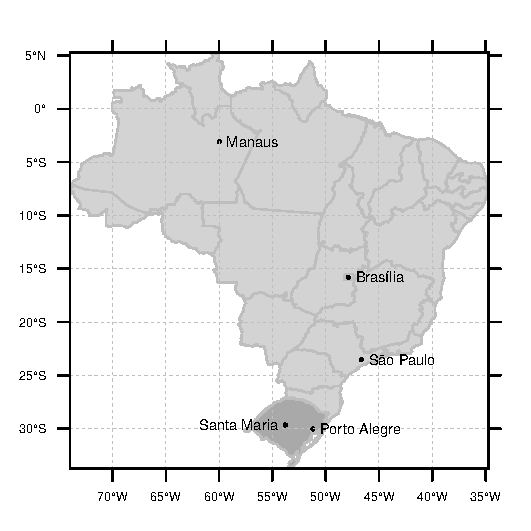
\includegraphics[width=90mm]{chap01FIG1a}
    \end{minipage}
    \begin{minipage}[b]{95mm}
      \subcaption{}
      \label{fig:points}
      \centering
      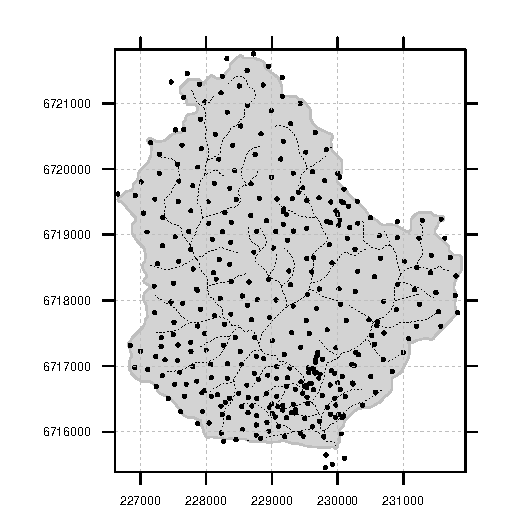
\includegraphics[width=90mm]{chap01FIG1b}
    \end{minipage}
  \caption{The study area. The top panel shows the location of the study area in the central region 
  of the southernmost Brazilian state, Rio Grande do Sul. The bottom panel uses a RapidEye image
  of the year of 2012 in perspective to give an overview of the land use and terrain features.
  A large collection of images of the study area are available at the web-page of the group
  \href{http://www.panoramio.com/group/130903}{Águas do Perau} on Panoramio.}
  \label{fig:intro-location}
\end{figure}

The geology of the study area is composed of three geological formations plus Quaternary deposits
\cite{GasparettoEtAl1988,MacielFilho1990,Sartori2009}. Consolidated sedimentary rocks (fluvial 
sandstone -- Caturrita Formation) of the Triassic period appear at elevations bellow \SI{\pm200}{\metre}.
Basic and acid igneous rocks (andesite-basalt and rhyolite-rhyodacite -- Serra Geral Formation) of the
Cretaceous period appear at elevations between \num{\pm200} and \SI{\pm350}{\metre}, and above 
\SI{\pm350}{\metre}, respectively. Between these rocks there are layers of consolidated sedimentary 
rocks (aeolian sandstone -- Botucatu Formation) of the Jurassic period. Unconsolidated colluvial 
deposits of igneous and sedimentary material eroded further upslope during the Quaternary period 
occur at elevations below \SI{\pm300}{\metre}, while recent fluvial deposits can be found close to 
drainages.

Current geomorphology is a result of erosive processes of the Tertiary and Quaternary, wherein the 
landscape sculpting was determined by alternations between humid, semi-arid and arid climates 
\cite{Sartori2009}. Landscape dissection is weak due to the current climate that favours the 
installation and maintenance of an exuberant vegetation \cite{Sartori2009,NascimentoEtAl2010}.
There are three large morphostructural units \cite{GasparettoEtAl1988,NascimentoEtAl2010}:

\begin{enumerate}[label=(\alph*)]
	\item the Planalto, with gently-rolling to slopping relief, composed predominately of 
	denudational forms with flat surfaces, convex tops, and gently rolling convex slopes, often 
	embedded in faults and/or fractures,

	\item the Rebordo do Planalto, with wide altimetric variation, steep slopes and abrupt 
	cliffs, composed predominately of denudational forms with convex, acute tops, presenting 
	straight slopes with large vertical drops often interrupted by terraces, generally embedded
	in faults and/or fractures, and

	\item the Depressão Periférica, composed of aggradational fluvial plains and denudational 
	forms, the last with convex tops and flat surfaces, presenting concave elongated slopes.
\end{enumerate}

The drainage network has a well defined pattern, generally regular, determined by the faults and/or
fractures \cite{Bortoluzzi1974,GasparettoEtAl1988,NascimentoEtAl2010}. In the lower areas, its
configuration is snake-like due to sediment deposition and fluvial erosion 
\cite{PaivaEtAl2001,SutiliEtAl2009}. Here the plain to gently-sloping, long, concave slopes favour the
occurrence of a 
water table close to the surface and the maintenance of perennial water streams. In the upper, 
undulating areas the rectilinear drainage network has little activity in periods of drought. Floods 
are characterized by high flow velocity and volume due to the steep slopes and \SI{\pm120}{\metre} 
vertical drop from the upper to the lower part of the catchment \cite{PaivaEtAl2001,SutiliEtAl2009}.

Land use for agrosylvopastoral production was intense in past times, resulting in severe soil 
degradation. Recent abandonment of many degraded areas allowed the regeneration of natural 
vegetation. The area occupied with forest and secondary vegetation nowadays is \SI{\pm60}{\percent},
specially in difficult to access areas, with steep slopes, shallow and stony soil 
\cite{SamuelRosaEtAl2011a}. Many of these areas are still used for livestock during some periods of
the year, which is negative for natural regeneration \cite{ScheneiderEtAl1978,HackEtAl2005}, and 
are traversed by old and degraded trails that drain rainwater. About \SI{\pm30}{\percent} of the 
area is used for agrosylvopastoral activities year-round, mainly extensive livestock, which relies 
on natural pastures in areas with deeper, less stony soil, and less sloping relief. Only a few 
agrosylvopastoral activities are carried out in areas with steep slops and shallow soil. Urban
settlements occupy only a small portion of the catchment, mainly close to drainages, the largest
settlements being in the southern region.

The soil in the study area started forming during the Triassic and have a strong dependency on the 
parent material \cite{NascimentoEtAl2010}. It is predominantly shallow (\SI{0.5}{\metre}, Neossolo 
and Cambissolo) due to the dominance of steep slopes, which result in soil formation rates being 
close to or lower than soil erosion rates \cite{DalmolinEtAl2006a}. Even in gently-slopping terrain
it is common to find shallow soils as a result of soil degradation \cite{Moser1990, MouraBueno2012}.
Deeper soil (\SI{>1}{\metre}, Argissolo and Planossolo) can be found in the Planalto, in the 
terraces of the Rebordo do Planalto, and in the small hills with gently-rolling slopes and alluvial 
plains of the Depressão Central \cite{Moser1990,MiguelEtAl2012}. Soil texture is finer and more 
homogeneous throughout the soil profile when the soil has developed from igneous rocks, where the 
presence of iron oxides gives a reddish colour to the soil \cite{MiguelEtAl2012}. Soil features in 
the alluvial plains are determined by seasonal or permanent water-logging, sedimentation, or both 
(Planossolo and Neossolo Flúvico). One such feature is the common presence of clay accumulation in
subsurface horizons due to argiluviation, preferential lateral erosion and, possibly, geological
discontinuities \cite{PieriniEtAl2002,MiguelEtAl2012}.

\subsection{Database}
\label{sec:intro-database}

The soil database used to develop the case studies is part of the \emph{Santa Maria dataset} 
(\autoref{apen:database}), a dataset composed of $n = 410$ soil observations made between \num{2004} 
and \num{2013} as part of different research projects. These projects aimed at producing semi-detailed
soil and land use maps (\scale{25000})
\cite{Pedron2005,Miguel2010,SamuelRosaEtAl2011a,MiguelEtAl2012,Samuel-RosaEtAl2013}, and predicting the
vulnerability of the topsoil to erosion \cite{MouraBueno2012,Miguel2013}. The Santa Maria dataset, which is
freely available at ISRIC World Soil Information Service
(\href{http://www.isric.org/data/wosis}{WoSIS}), and is fully documented at the end of this thesis 
(\autoref{apen:database}), is composed of three subsets, but only two of them are used here 
(\reffig{intro-database}).

\begin{figure}[!ht]
\centering
\includegraphics{fig/chap00-intro-database}
\caption{Spatial distribution of the $n = 340$ (black) and $n = 10$ (red) soil observations from 
the Santa Maria dataset used in this thesis. The drainage network is shown in the background to 
give an idea of how sampling locations are related to terrain features.}
\label{fig:intro-database}
\end{figure}

The first dataset ($n = 340$) was produced using purposively selected observation locations (free 
survey). The main goal of the researchers was to obtain a sample that they understood as being 
representative of the different landforms, land uses, and soil taxa present in the study area. They 
also wanted the sample to cover the entire study area. At the observation locations, they defined 
an area of \SI{\approx100}{\metre\squared} within which they opened three soil pits. Soil samples 
were collected up to a depth of \SI{20}{\centi\metre}. The resulting sampling depth varies from 
\num{2} to \SI{20}{\centi\metre}, with a mean of \SI{17}{\centi\metre}. Soil samples from the three 
pits were used to produce a composite sample which was used for laboratory analysis. Georeferencing 
took place in the field using a GNSS signal receiver with a horizontal precision of more than 
\SI{\pm8}{\metre} positioned approximately at the centre of the sampling area. When the GNSS signal 
was affected by vegetation biomass, terrain features and satellite configuration, resulting in a 
horizontal positional error larger than \SI{\pm8}{\metre}, georeferencing was carried out in the 
office using \SI{1}{\metre} spatial resolution Google Earth\textregistered{} satellite image with 
a positional horizontal error of less than \SI{\pm6}{\metre}.

The second dataset ($n = 10$) contains data from the uppermost A horizon of modal soil profiles 
whose locations were purposively selected after the observations of the first dataset had been made, 
and a preliminary area-class soil map had been produced. The researchers aimed at locations that 
they understood as being most representative of the soil mapping units depicted in the area-class 
soil map. A single soil sample was taken from the each described soil horizon and used for 
laboratory analysis. The resulting depth of the uppermost A horizons varies from \num{12} to 
\SI{30}{\centi\metre}, with a mean of \SI{22.6}{\centi\metre}. Georeferencing was carried out as 
described above, the difference being that GNSS signal receiver was positioned at the observation 
location.

Four soil properties contained in the Santa Maria dataset are explored in this thesis: clay content
(CLAY, \si{\gram\per\kilo\gram}), organic carbon content (ORCA, \si{\gram\per\kilo\gram}), effective
cation exchange capacity (ECEC, \si{\milli\mole\per\kilo\gram}), and bulk density (BUDE, 
\si{\mega\gram\per\cubic\metre}). CLAY was determined by the pipette method. ORCA was determined 
using wet digestion. ECEC was calculated as the sum of exchangeable bases plus exchangeable acidity.
BUDE was determined using the core method. The first three soil properties were selected because 
they were expected to present different patterns of spatial variation and correlation with the 
dominant factors of soil formation in the study area: organisms (\textit{O}), relief (\textit{R}), 
and parent material (\textit{P}). CLAY was presumed to have a stronger relation with \textit{P}, 
while ORCA was expected to be more correlated with \textit{O}. Because the soils of the study area 
were strongly eroded due to intense agriculture in the 20th century, both CLAY and ORCA were also 
expected to be closely related with \textit{R}. Finally, ECEC was expected to be strongly correlated
with \textit{P} and \textit{O}, which is supported by its natural relationship with both CLAY and 
ORCA. BUDE was selected because it was the only soil property that approximately follows a normal 
frequency distribution, while the other three have a right-tailed frequency distribution 
(\autoref{intro-soil-properties}). The main weakness of the BUDE data is that it is available at 
only $n = 282$ observations due to soil stoniness.

\begin{figure}[!ht]
\centering
\begin{minipage}[b]{63mm}
\subcaption{}
\centering
\includegraphics{fig/chap00-intro-clay}
\end{minipage}
\begin{minipage}[b]{63mm}
\subcaption{}
\centering
\includegraphics{fig/chap00-intro-orca}
\end{minipage}
\begin{minipage}[b]{63mm}
\subcaption{}
\centering
\includegraphics{fig/chap00-intro-ecec}
\end{minipage}
\begin{minipage}[b]{63mm}
\subcaption{}
\centering
\includegraphics{fig/chap00-intro-bude}
\end{minipage}
\caption{The four soil properties explored in this thesis: (a) clay content, (b) organic carbon 
content, (c) effective cation exchange capacity, and (d) bulk density. Each panel shows the sample 
histogram and summary statistics of the soil properties in their original scale ($\lambda = 1$), as 
well as the theoretical probability density function so that we can assess how good is the fit of 
the normal distribution to the data -- a product of the \Rpackage{pedometrics}.}
\label{fig:intro-soil-properties}
\end{figure}

A list of more than \num{100} covariates were used in this thesis. All of them were derived from 
five freely available sources: area-class soil maps, digital elevation models, geological maps,
land use maps, and orbital images. Each of these sources was explored in two levels of spatial 
detail, here defined by the data sources and/or production methods, which demand different amounts 
of resources (time, workforce, budget, technology, etc.). Specifically, the level of spatial detail 
of a covariate is a function of the components of its production process such as the cartographic 
ratio, spatial sampling support, number and diversity of data sources explored, and quantity of 
spatial data used. This definition of spatial detail is broader than that of spatial resolution
or spatial scale, and should not be confounded with spatial support \cite{WebsterEtAl2007} or 
thematic detail \cite{Rossiter2000}.

The first area-class soil map was published at a \scale{100000} \cite{AzolinEtAl1988}, while the 
second was prepared at the more detailed \scale{25000} \cite{MiguelEtAl2012}. The first digital 
elevation model is the result of interpolating the contour lines of the most recent topographic maps
produced by the Brazilian Army (\scale{25000}) \cite{DSG1980,DSG1992,DSG1992a}, while second 
digital elevation model is the well known SRTM DEM (3 arc-seconds \SI{\approx90}{\metre} spatial 
resolution) produced by NASA’s Jet Propulsion Laboratory in collaboration with the National 
Geospatial-Intelligence Agency \cite{RodriguezEtAl2006}. Data on geology and soil parent material 
comes from most recent geological maps published in the \scales{25000}{50000} 
\cite{MacielFilho1990,GasparettoEtAl1988}. The land use map of the year of 1980 comes from the most 
recent topographic 
map produced by the Brazilian Army already mentioned above. The second land use map refers to the 
years of 2008 and 2009, and was prepared at a \scale{2000} \cite{SamuelRosaEtAl2011a}. The less 
detailed satellite image was acquired by the Landsat-5 Thematic Mapper on December 26, 2010, while
the more detailed satellite image comes from the RapidEye constellation, acquired on November 16, 
2012. A comprehensive description of these covariates and their processing is presented in the 
end of this thesis (\autoref{apen:database}).

\subsection{Outline}
\label{sec:thesis-outline}

This thesis is composed of five chapters: this \emph{General Introduction}, where I present the scope 
of the thesis, three core chapters where I address the objectives and research questions presented
in \refsec{thesis-objectives}, and the last, a \emph{General Conclusion} (\autoref{chap:conclusion})
of the work that I developed during the last four years. The second chapter (\autoref{chap:chapter01}) 
is based on an article published in the peer reviewed journal \geoderma. There I compare linear 
soil-mapping models calibrated using covariates available in two levels of detail, with and without 
taking the spatial dependence of the residuals into account (Questions 1a-c).

The third (\autoref{chap:chapter02}) and fourth chapters (\autoref{chap:chapter03}) are based on 
manuscripts to be submitted to peer reviewed journals, both dealing with the second objective of this
thesis. In the former I evaluate if improving a popular algorithm used to optimize sample configurations
for spatial trend estimation results in more accurate spatial predictions (Questions 2a and 2f). In the
last I compare five methods for designing sample configurations on how they affect estimated model 
parameters and prediction accuracy (Questions 2b and 2e). I also present an algorithm for optimizing 
sample configurations for identifying and estimating the spatial trend and variogram model, and making
spatial predictions (Question 2d). Finally, I evaluate the gain in prediction accuracy when a sample 
configuration is optimized assuming the form of the model to be known (Question 2c).

This thesis also includes a through description of the soil and covariate databases 
(\autoref{apen:database}), and a verbal representation of the conceptual model of pedogenesis 
(\autoref{apen:pedogenesis}), both summarized above in \refsec{database}. \autoref{apen:spsann} contains
a description of the \Rpackage{spsann}, which I designed for the optimization of sample configurations
using spatial simulated annealing. Finally, \autoref{apen:pedometrics} presents a description of the 
\Rpackage{pedometrics}, which includes miscellaneous functions.

All chapters can be read separately, which means that there might be some overlap between them, 
i.e. repeated information. However, there are clear links between this introductory chapter 
and the concluding chapter. \autoref{chap:chapter02}, \autoref{chap:chapter03}, and \autoref{apen:spsann} 
also are closely connected. References to specific sections of other chapters are common. All literature
references are presented under a unique \emph{Bibliographic References} chapter (\autoref{chap:references})
at the end of this thesis.
